% =====================================================================================
%  SQD with configuration recovery on ROQUO (GB200) — UHF & RHF on Fe-S active spaces
%  Self-contained Overleaf/LaTeX summary for presentation (2026-07-08).
%
%  Compile: pdflatex presentation.tex  (twice, for references).
%  Figures expected alongside this file (see \graphicspath); placeholders are noted
%  where a run is still in progress.
% =====================================================================================
\documentclass[11pt]{article}
\usepackage[margin=1in]{geometry}
\usepackage{graphicx}
\usepackage{booktabs}
\usepackage{amsmath}
\usepackage{xcolor}
\usepackage{listings}
\usepackage{hyperref}
\usepackage{longtable}
\hypersetup{colorlinks=true, linkcolor=blue, urlcolor=blue}
\graphicspath{{./}{figures/}}

\lstset{basicstyle=\ttfamily\footnotesize, breaklines=true, frame=single,
        backgroundcolor=\color{gray!8}, columns=fullflexible}

\title{\textbf{Quantum--Classical SQD with Configuration Recovery on ROQUO (GB200)}\\
       \large UHF and RHF closed-loop pipeline on Fe$_2$S$_2$ (40q) and Fe$_4$S$_4$ (72q)}
\author{QCSC / \texttt{qcsc-prefect} --- branch \texttt{kk/feature/uhf}}
\date{2026-07-08}

\begin{document}
\maketitle

\begin{abstract}
We report a closed-loop Sample-based Quantum Diagonalization (SQD) pipeline with
self-consistent \emph{configuration recovery}, run end-to-end through Prefect on the RIKEN
\textbf{ROQUO} GB200 GPU supercomputer. Quantum samples are drawn from IBM hardware
(\texttt{ibm\_kobe}); the selected-CI diagonalization runs on the GB200 GPU via a newly built
\texttt{nvc++} solver (\texttt{diag-gpu}). We demonstrate the recovery effect for both the
unrestricted (UHF) and restricted (RHF) reference on two iron--sulfur active spaces:
Fe$_2$S$_2$ (40 qubits, 30e/20o) and Fe$_4$S$_4$ (72 qubits, 54e/36o), benchmarked against
UHF, UCCSD, and CCSD(T). All orchestration is Prefect-native (no bespoke driver): the flow
submits each GPU solve as a Slurm job and polls it, mirroring the existing Fugaku (PJM) and
Miyabi (PBS) targets.
\end{abstract}

\tableofcontents

% =====================================================================================
\section{What was done (since Wed.\ 2026-07-01)}
% =====================================================================================
Two threads of work: (i) a molecule-parametrized \emph{recovery} harness with per-iteration
telemetry, and (ii) bringing the pipeline up on ROQUO's GB200 GPUs through Prefect's Slurm
target, including building the GPU solver with the newly installed \texttt{nvc++}. The headline
scientific result is the first 72-qubit (Fe$_4$S$_4$) SQD recovery trajectory on GB200 GPU.

\paragraph{Highlights.}
\begin{itemize}
  \item \textbf{Per-iteration recovery telemetry.} Added a \texttt{recovery\_trace} to the SQD
        walker so every configuration-recovery pass records energy, subspace dimension, spin
        density ($2S_z$), useful-determinant fraction, and occupancies --- previously only the
        best pass survived, so the recovery \emph{curve} was unrecoverable.
  \item \textbf{Molecule-parametrized harness.} One code path drives both Fe$_2$S$_2$ and
        Fe$_4$S$_4$ (select via \texttt{FE\_MOL}); ``sample once, reuse'' persists the 5\,M-shot
        pool and re-diagonalizes offline (\texttt{quantum\_source="saved"}).
  \item \textbf{ROQUO GPU build.} Built \texttt{diag-gpu}/\texttt{diag-gpu\_uhf} with
        \texttt{nvc++} 26.5 (\texttt{-cuda -gpu=cc100}) for GB200 (sm\_100) --- the previously
        blocking \texttt{\_\_syncwarp} issue is a non-problem for \texttt{nvc++}.
  \item \textbf{Prefect Slurm target for GPU.} Extended \texttt{create\_blocks.py} and the Slurm
        adapter so a GPU solve is submitted as an \texttt{sbatch} job (\texttt{--gres=gpu:1},
        \texttt{module load cuda/13.2 hpcx/2.50}, launched with \texttt{srun --gpu-bind=closest}
        over PMIx). The orchestrator only submits and polls (\texttt{sacct}), keeping it light.
  \item \textbf{References.} UHF/UCCSD/CCSD(T) computed from the FCIDUMP (convergence hardened:
        \texttt{max\_cycle=300}, DIIS, level shift). HCI is skipped above 24 orbitals
        (intractable at 72q); DMRG deferred to a block2 reference environment.
\end{itemize}

% =====================================================================================
\section{ROQUO: features, and how it compares to Miyabi}
% =====================================================================================
\subsection{ROQUO at a glance}
\begin{longtable}{@{}p{0.28\textwidth}p{0.66\textwidth}@{}}
\toprule
System & Supercomputer ROQUO (RIKEN R-CCS, Kobe); quantum--HPC integration platform \\
Compute nodes & 135$\times$ NVIDIA GB200 NVL4 (8 racks qr01--qr08) \\
Per node & 2$\times$ Grace (Arm Neoverse-V2, 144 cores, SMT off) + 4$\times$ Blackwell GPU
           (GB200 NVL4, Grace--Blackwell NVLink-coupled) \\
GPU arch & Blackwell, CUDA compute capability 10.0 (build \texttt{sm\_100} / \texttt{cc100}, CUDA 13) \\
CPU arch & \textbf{compute nodes arm64 (aarch64)}; \textbf{login nodes x86\_64} --- build on a compute node \\
Interconnect & Quantum-X800 InfiniBand (4 links/node); full BW in-rack, 4:1 across racks \\
Scheduler & Slurm (cluster \texttt{roquo}, default partition \texttt{roquo}); MPI = HPC-X (OpenMPI\,5 / PMIx) \\
Node plans & auto-round to qtr (1 GPU/36c/400G), half (2/72/800), full (4/144/1600) \\
Storage & \texttt{/home} (Lustre-backed, persistent); \texttt{\$SLURM\_SCRATCH} (per-job local NVMe, 7\,TB) \\
OS & Rocky Linux 9.8 \\
\bottomrule
\end{longtable}

\subsection{Similar to / different from Miyabi}
\textbf{Similar:} both are Grace(+GPU) systems; both are driven by the \emph{same} Prefect
executor pattern --- the flow orchestrates and submits \emph{each} solve as a scheduler job,
then polls terminal status. The domain code (SQD flow, recovery loop, integral build) is
identical across targets.

\textbf{Different:}
\begin{itemize}
  \item \textbf{Scheduler:} ROQUO uses \textbf{Slurm} (\texttt{sbatch}/\texttt{srun}/\texttt{sacct},
        PMIx MPI); Miyabi uses \textbf{PBS} (\texttt{qsub}/\texttt{qstat}); Fugaku uses \textbf{PJM}
        (\texttt{pjsub}). We added a first-class \texttt{slurm} \texttt{hpc\_target} alongside the
        existing \texttt{miyabi}/\texttt{fugaku} ones.
  \item \textbf{GPU:} ROQUO is Blackwell (\texttt{sm\_100}), whole-node = 4 GPUs; the SBD GPU
        binary is built with \texttt{nvc++} and launched one MPI rank per GPU.
  \item \textbf{Resource model:} ROQUO auto-rounds GPU/CPU/memory to node plans (qtr/half/full);
        no explicit ``select'' string as on PJM/PBS.
  \item \textbf{Arch split:} login x86\_64 vs compute aarch64 --- the Prefect orchestrator must run
        on a compute node (aarch64 venv), unlike a single-arch cluster.
\end{itemize}

% =====================================================================================
\section{The closed-loop pipeline (UHF and RHF)}
% =====================================================================================
The pipeline is identical for UHF and RHF; the reference (and thus the LUCJ ansatz + the
diagonalizer binary) is selected by the solver block's \texttt{--method}.

\begin{enumerate}
  \item \textbf{Integrals \& ansatz seed.} From the FCIDUMP, build (U)HF + (U)CCSD; the CCSD
        amplitudes seed the LUCJ circuit parameters.
  \item \textbf{Quantum sampling (once).} Run the LUCJ circuit on \texttt{ibm\_kobe} (5\,M shots,
        5 batches; DD (XY4) + measurement twirling). Persist the merged bitstring pool to Lustre
        --- \emph{sampled once, reused forever} (\texttt{quantum\_source="saved"}).
  \item \textbf{Configuration recovery (multi-iteration).} For each pass: recover configurations
        from the saved pool using the current occupancies, Hamming-weight post-select, subsample a
        subspace of dimension \texttt{sqd\_dim}=$3\times10^8$, and diagonalize on GB200 GPU. Feed
        the new occupancies into the next pass. Each pass is a \texttt{sbatch} GPU job.
  \item \textbf{References.} UHF/UCCSD/CCSD(T) as flat comparison lines.
  \item \textbf{Figures.} Energy vs recovery iteration + diagnostics; cross-system view.
\end{enumerate}

\subsection{How to run it (precise, end-to-end)}
\begin{lstlisting}[language=bash]
# --- ROQUO login (x86_64) -> pull code, then work on a compute node (aarch64) ---
ssh -i ~/.ssh/roquo_ed25519 q0000219@login.roquo.qc.r-ccs.riken.jp
cd ~/qcsc-prefect && git pull origin kk/feature/uhf

# 0) One-time: build the GPU solver on a COMPUTE node (aarch64, nvc++)
srun --account=q0000219 --gres=gpu:1 --time=00:25:00 bash -lc '
  NV=/opt/nvidia/hpc_sdk/Linux_aarch64/26.5
  export PATH=$NV/compilers/bin:$NV/comm_libs/hpcx/bin:$PATH
  export OMPI_CXX=nvc++
  cd ~/qcsc-prefect/algorithms/sbd/native
  CCCOM=mpic++ CCFLAGS="-std=c++17 -mp -cuda -fast -gpu=mem:unified,cc100 -DSBD_THRUST" \
    SYSLIB="/usr/lib64/libopenblaso.so.0 -lgfortran" bash build_sbd_gpu.sh          # diag-gpu
  UHF=1 CCCOM=mpic++ CCFLAGS="-std=c++17 -mp -cuda -fast -gpu=mem:unified,cc100 -DSBD_THRUST -D_UHF" \
    SYSLIB="/usr/lib64/libopenblaso.so.0 -lgfortran" bash build_sbd_gpu.sh          # diag-gpu_uhf
'

# 1) Credentials (gitignored): sweep/.env.local with IBM_API_KEY / IBM_CRN / IBM_BACKEND=ibm_kobe
# 2) Sample once on kobe (UHF or RHF); pool persists on Lustre
cd ~/qcsc-prefect/algorithms/sbd/sweep
METHOD=uhf sbatch --gres=gpu:1 --time=03:00:00 run_fe4s4_sample_roquo.sh   # (RHF: METHOD=rhf)

# 3) Multi-iteration GPU recovery from the saved pool (each solve = its own sbatch GPU job)
METHOD=uhf FE4S4_RECSTEPS=5 FE4S4_SQD_DIM=300000000 FE4S4_POOL=<persisted_pool.npz> \
  sbatch --gres=gpu:1 --time=04:00:00 run_fe4s4_gpu_roquo.sh                # (RHF: METHOD=rhf)

# 4) References + figures
sbatch --gres=gpu:1 run_fe4s4_refs_roquo.sh        # UHF/UCCSD/CCSD(T) -> runs/fe4s4_refs.json
python fe_twopanel_plot.py                          # two-panel figure
\end{lstlisting}

\paragraph{Key ROQUO-specific settings (baked into the runners).}
\begin{itemize}
  \item \texttt{--hpc-target slurm --solver-mode gpu --slurm-gres gpu:1}; launcher \texttt{srun},
        MPI options \texttt{--gpu-bind=closest} (PMIx).
  \item \texttt{diag-gpu} is an MPI binary: \emph{must} launch under \texttt{srun}/\texttt{mpirun}
        (one rank per GPU); it OOMs if a single 72q solve is split across ranks, so one solve per
        GPU. \texttt{n\_batches=1} (concurrent solves on one GPU OOM).
  \item \texttt{PREFECT\_HOME} on Lustre (pool persistence); \texttt{PREFECT\_API\_REQUEST\_TIMEOUT=600}
        (long child-solve polls exceed the 60\,s default); Prefect telemetry disabled.
\end{itemize}

% =====================================================================================
\section{Results}
% =====================================================================================
\subsection{Fe$_4$S$_4$ (72 qubits): UHF recovery on GB200 GPU}
The UHF-SQD energy drops from $-326.197$ Ha (iteration 1) and converges by iteration~3 to
$\approx -326.519$ Ha --- about \textbf{520\,mHa below the UHF reference}, recovering
$\sim$44\% of the UHF$\rightarrow$CCSD(T) correlation gap on a full $3\times10^8$-dimensional
subspace ($2S_z=0$ throughout). Each solve took $\sim$65--400\,s on one GB200.

\begin{table}[h]\centering
\begin{tabular}{@{}lrrrrr@{}}
\toprule
 & \multicolumn{5}{c}{Fe$_4$S$_4$ UHF-SQD recovery iteration (Ha)} \\
\cmidrule(l){2-6}
Step & 1 & 2 & 3 & 4 & 5 \\
\midrule
$E$ & $-326.1972$ & $-326.4973$ & $-326.5190$ & $-326.5085$ & $-326.5138$ \\
\bottomrule
\end{tabular}
\caption{Fe$_4$S$_4$ UHF-SQD recovery trajectory (sqd\_dim $=3\times10^8$, GB200 GPU).
References: UHF $-325.9987$, UCCSD $-326.8678$, CCSD(T) $-327.1762$ Ha.}
\end{table}

\begin{figure}[h]\centering
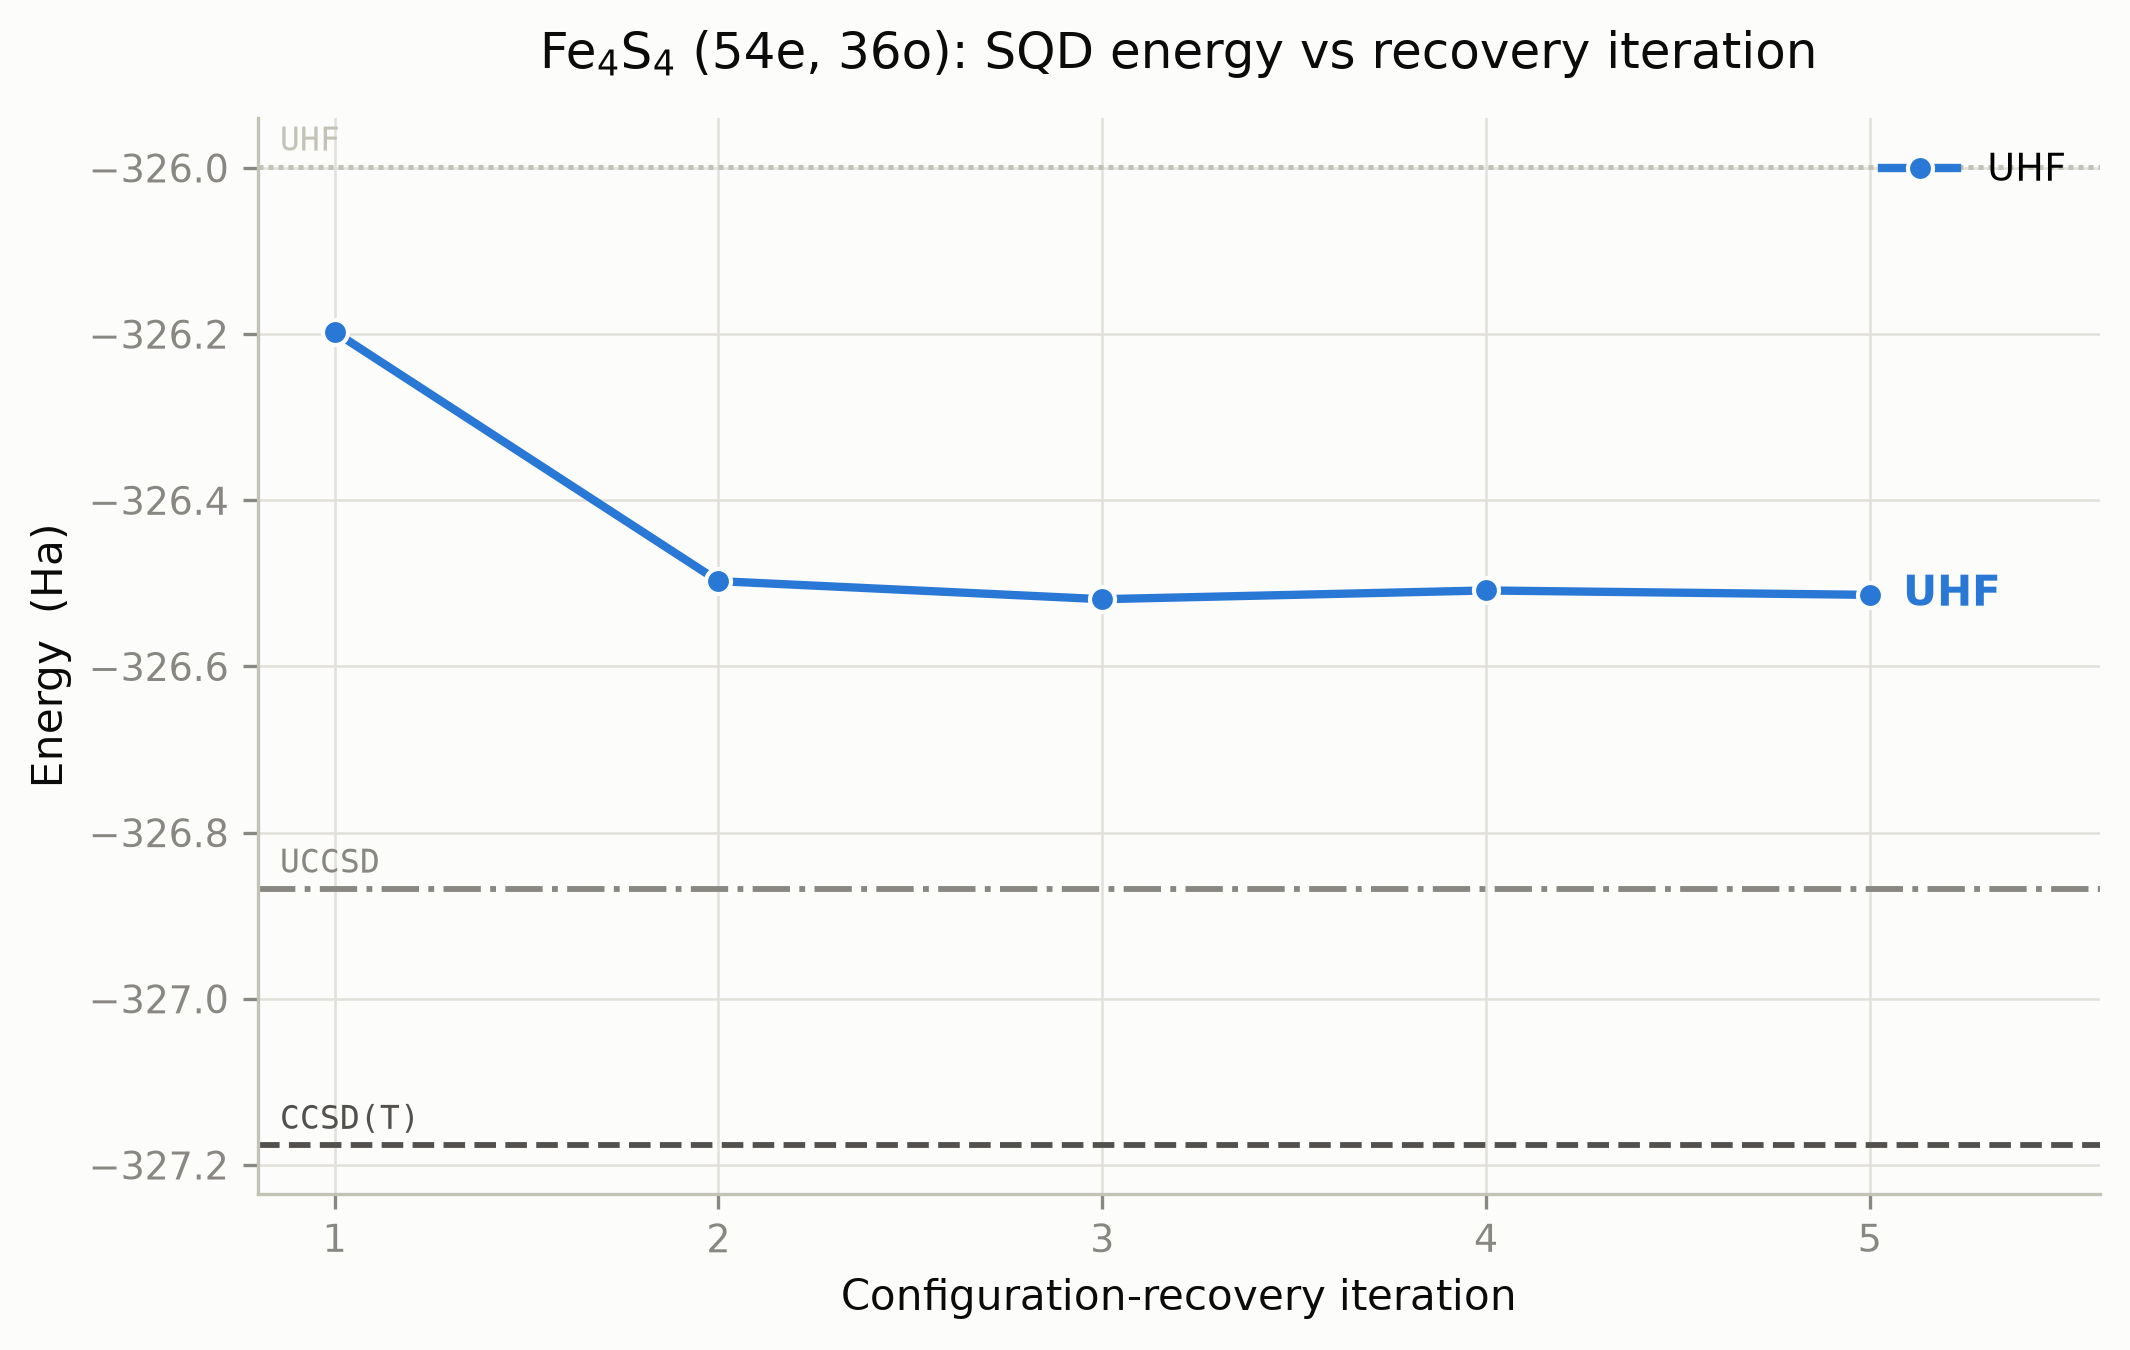
\includegraphics[width=0.9\textwidth]{fe4s4_energy_vs_iter.png}
\caption{\textbf{Fe$_4$S$_4$ (72q) UHF-SQD energy vs configuration-recovery iteration} on GB200
GPU. Blue: SQD recovery curve. Dashed/dotted lines: UHF, UCCSD, CCSD(T) references. The recovery
loop pulls the energy sharply below UHF within $\sim$3 iterations, toward the correlated
references. \emph{[Figure: \texttt{fe4s4\_energy\_vs\_iter.png}]}}
\end{figure}

\begin{figure}[h]\centering
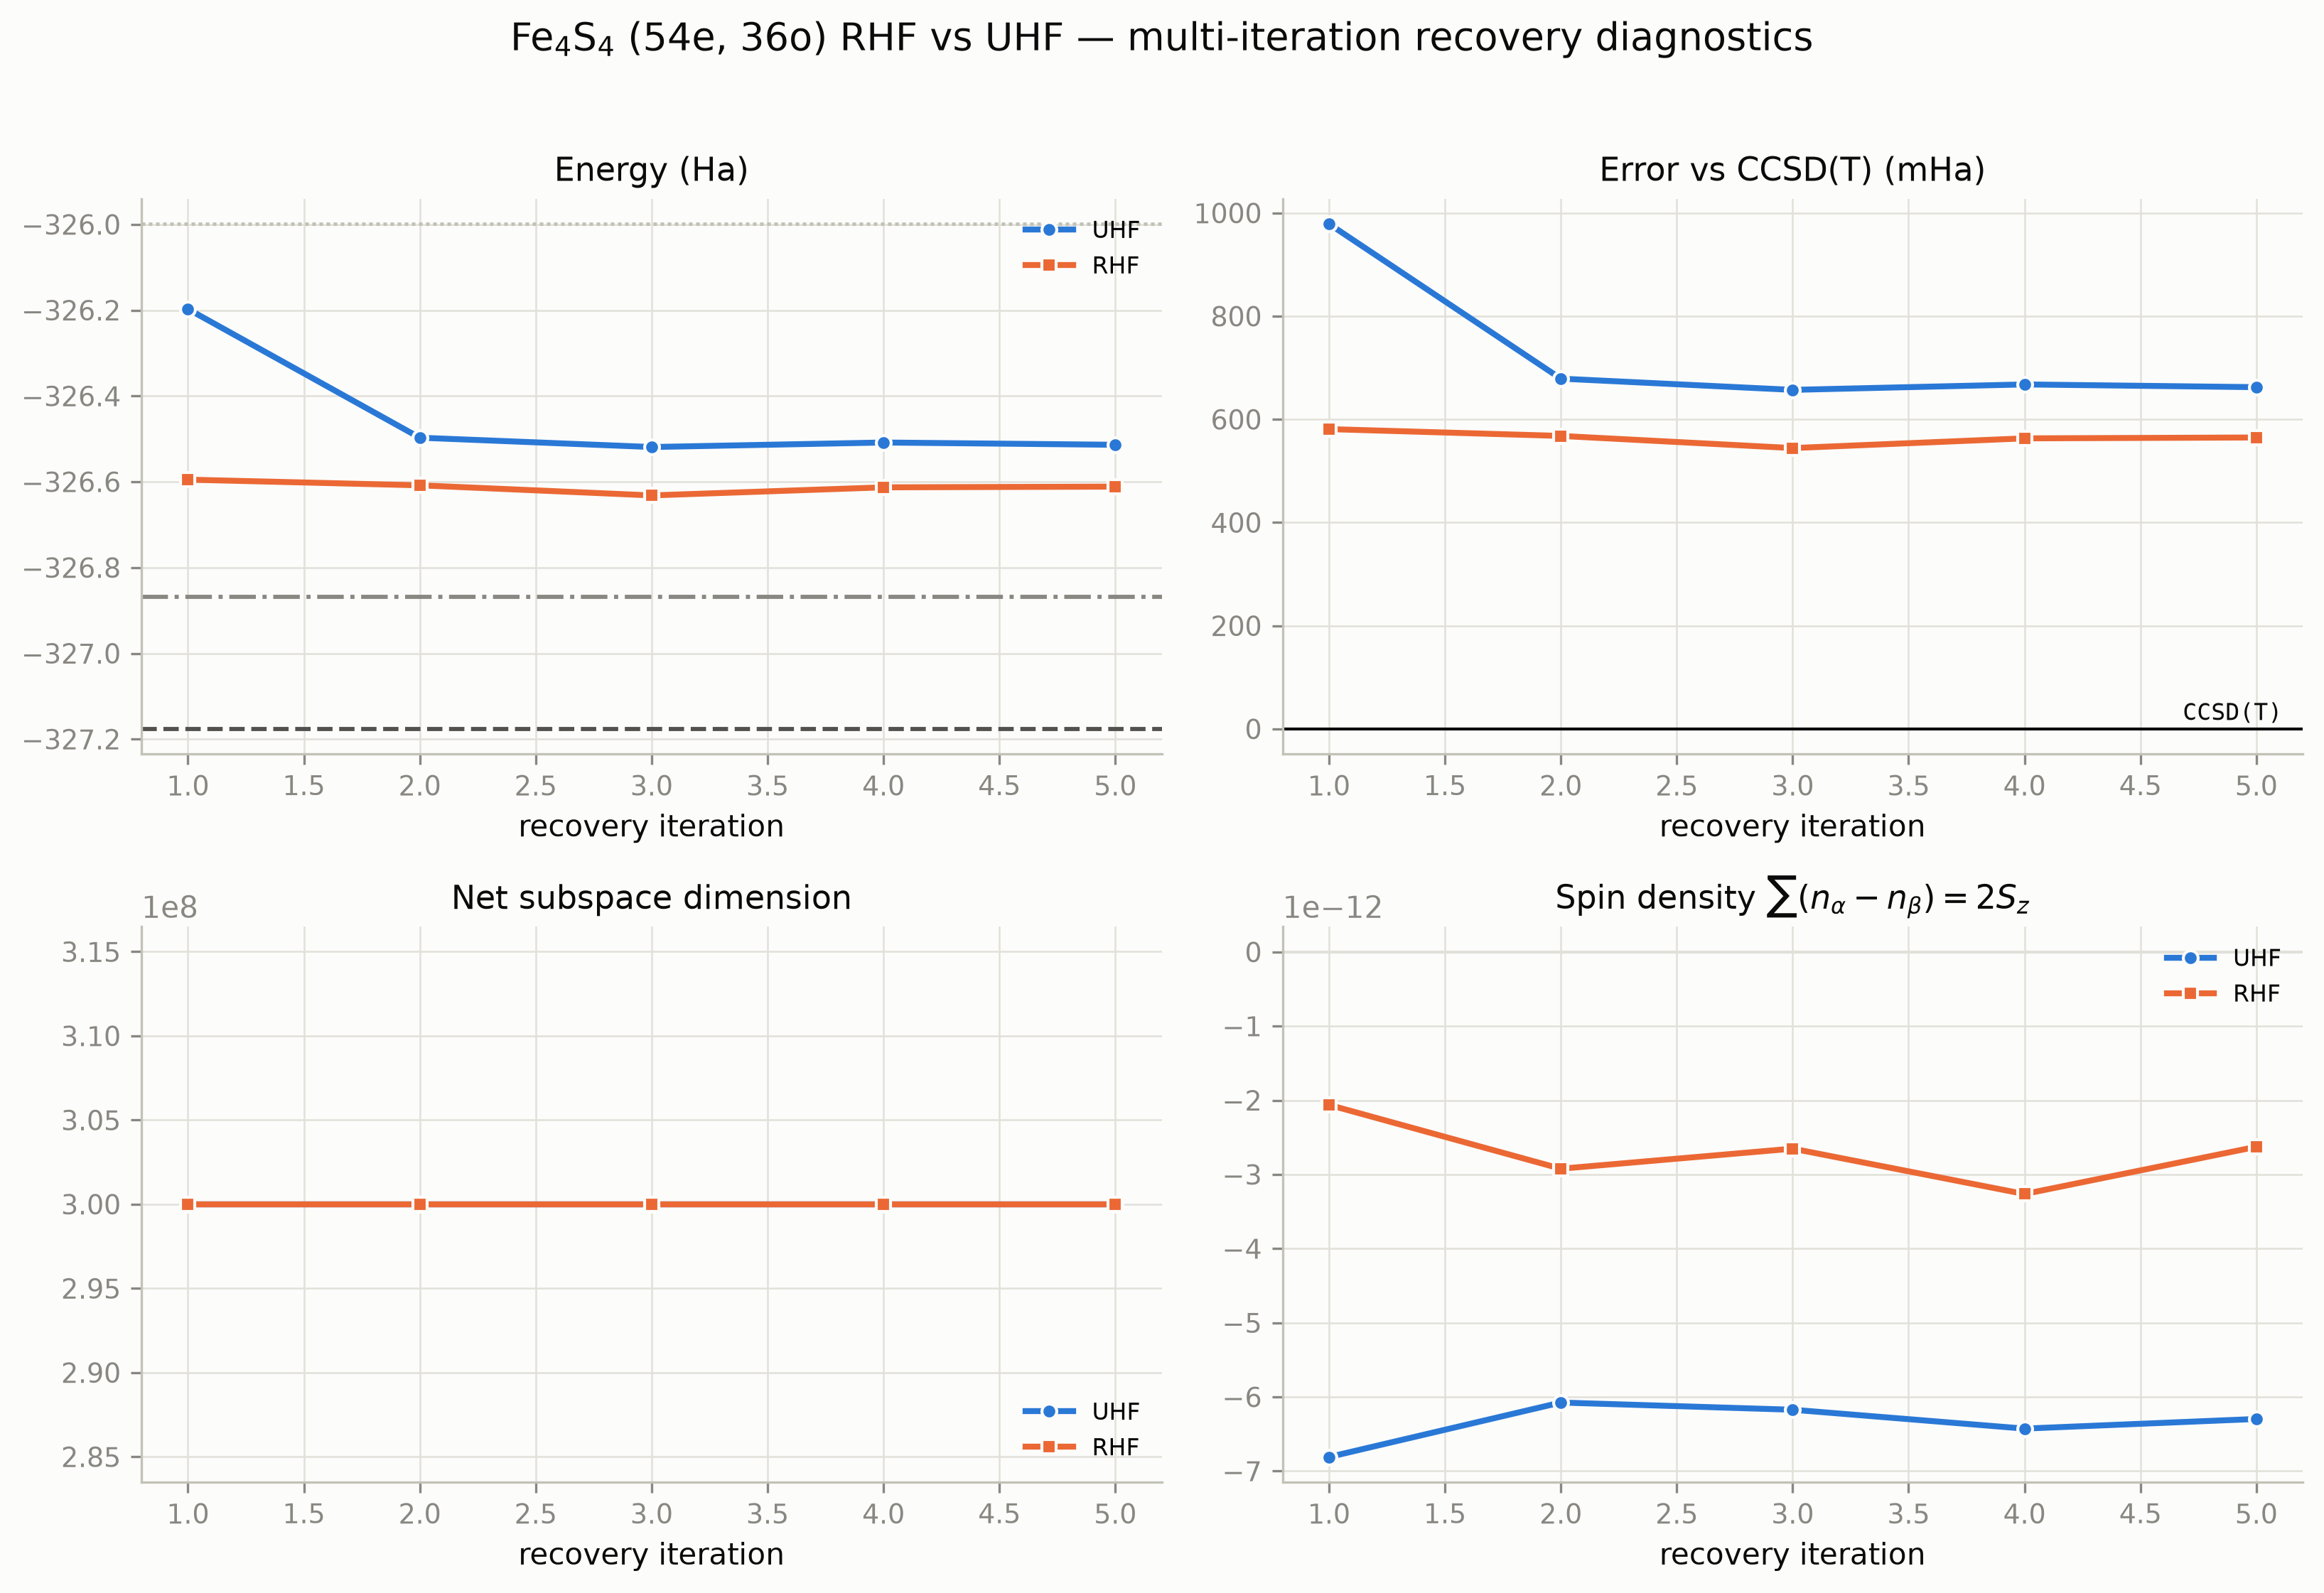
\includegraphics[width=0.95\textwidth]{fe4s4_panels.png}
\caption{\textbf{Fe$_4$S$_4$ diagnostics per recovery iteration:} energy; error vs CCSD(T) (mHa);
net subspace dimension ($3\times10^8$); spin density $\sum(n_\alpha-n_\beta)=2S_z$ ($\approx0$,
confirming the singlet). \emph{[Figure: \texttt{fe4s4\_panels.png}]}}
\end{figure}

\subsection{Two-system view: Fe$_2$S$_2$ (40q) and Fe$_4$S$_4$ (72q)}
Figure~\ref{fig:twopanel} is the summary comparison: both references (UHF blue, RHF orange) and
both active spaces, each panel on its own energy axis (the systems differ by $\sim$210\,Ha in
absolute energy). It shows the central result in one place --- SQD configuration recovery pulls
the energy well below the mean-field (UHF) reference toward the correlated CCSD(T) anchor on
\emph{both} a 40-qubit and a 72-qubit iron--sulfur system, and the restricted (RHF) reference
recovers slightly deeper than the unrestricted (UHF) one in both cases.

\begin{figure}[h]\centering
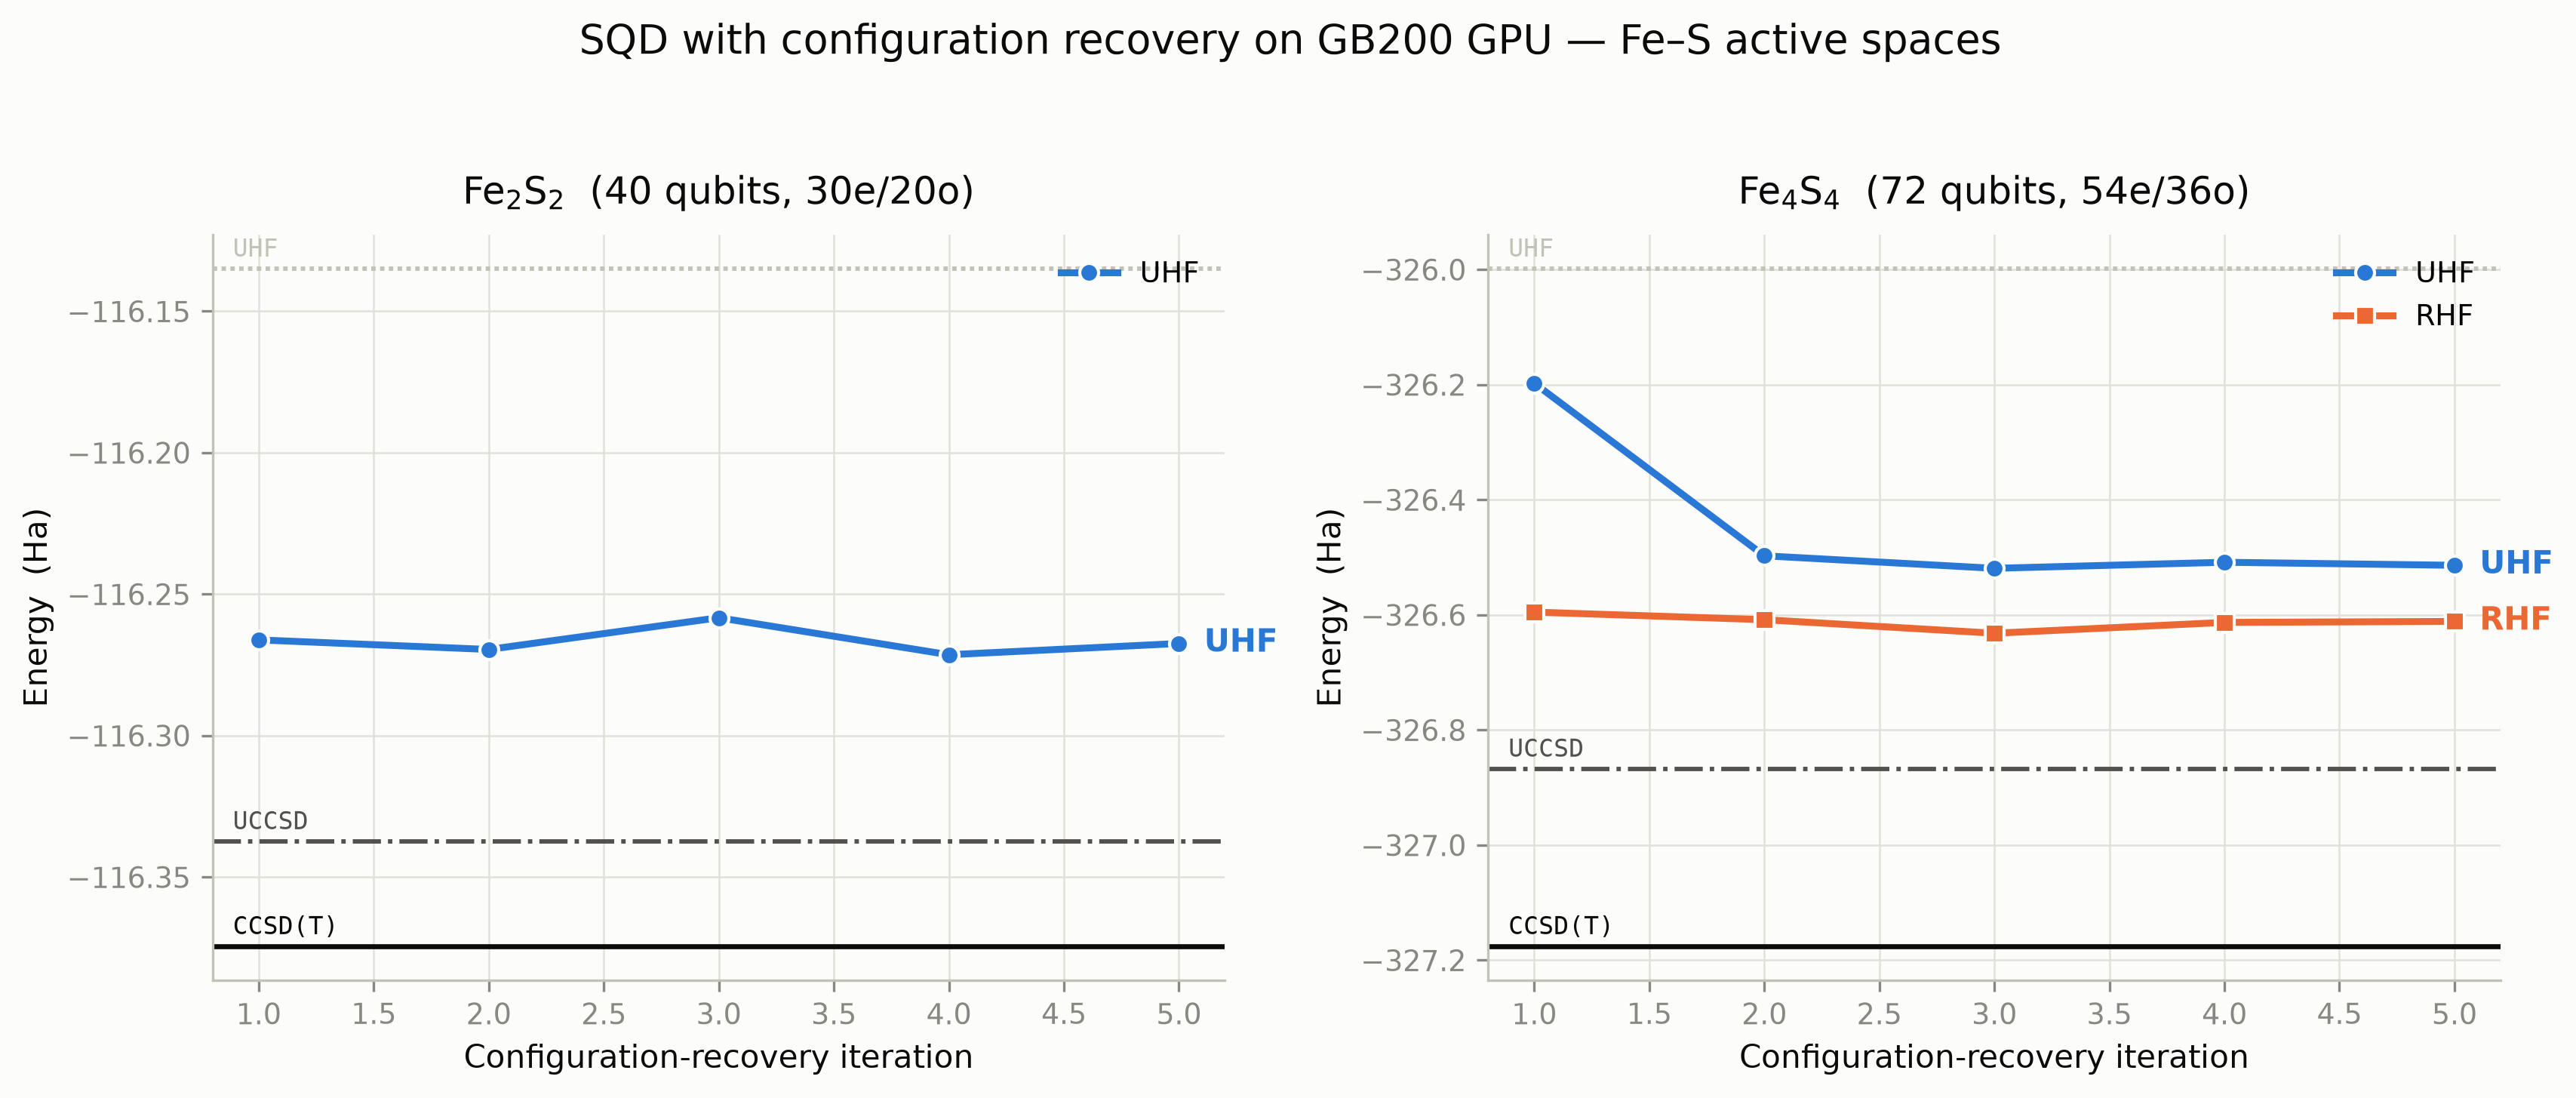
\includegraphics[width=0.98\textwidth]{fe_twopanel.png}
\caption{\textbf{SQD recovery on GB200 GPU across two Fe--S active spaces.} \emph{Left:}
Fe$_2$S$_2$ (40q) UHF- and RHF-SQD recovery curves vs UHF/UCCSD/CCSD(T). \emph{Right:}
Fe$_4$S$_4$ (72q), same. Blue = UHF-SQD, orange = RHF-SQD. Each panel has its own energy axis.
\emph{[Figure: \texttt{fe\_twopanel.png}]}}
\label{fig:twopanel}
\end{figure}

\subsection{Fe$_4$S$_4$ (72q): RHF vs UHF recovery}
The RHF pipeline is identical to UHF with \texttt{--method rhf} (RHF reference, restricted
diagonalizer). RHF was sampled independently on \texttt{ibm\_kobe} (5\,M shots) and its
5-iteration GPU recovery converges to $-326.632$ Ha --- notably \emph{below} the UHF-SQD result
($-326.519$), i.e.\ on this active space the restricted reference yields a slightly deeper
recovered energy. Both curves lie well below UHF, between UHF and UCCSD relative to CCSD(T).

\begin{table}[h]\centering
\begin{tabular}{@{}lrrrrrr@{}}
\toprule
Ref & it.1 & it.2 & it.3 & it.4 & it.5 & best \\
\midrule
UHF-SQD & $-326.197$ & $-326.497$ & $-326.519$ & $-326.509$ & $-326.514$ & $\mathbf{-326.519}$ \\
RHF-SQD & $-326.595$ & $-326.608$ & $-326.632$ & $-326.613$ & $-326.611$ & $\mathbf{-326.632}$ \\
\bottomrule
\end{tabular}
\caption{Fe$_4$S$_4$ (72q) RHF vs UHF SQD recovery trajectories (Ha; sqd\_dim $=3\times10^8$,
GB200 GPU). References: UHF $-325.9987$, UCCSD $-326.8678$, CCSD(T) $-327.1762$ Ha.}
\end{table}

\begin{figure}[h]\centering
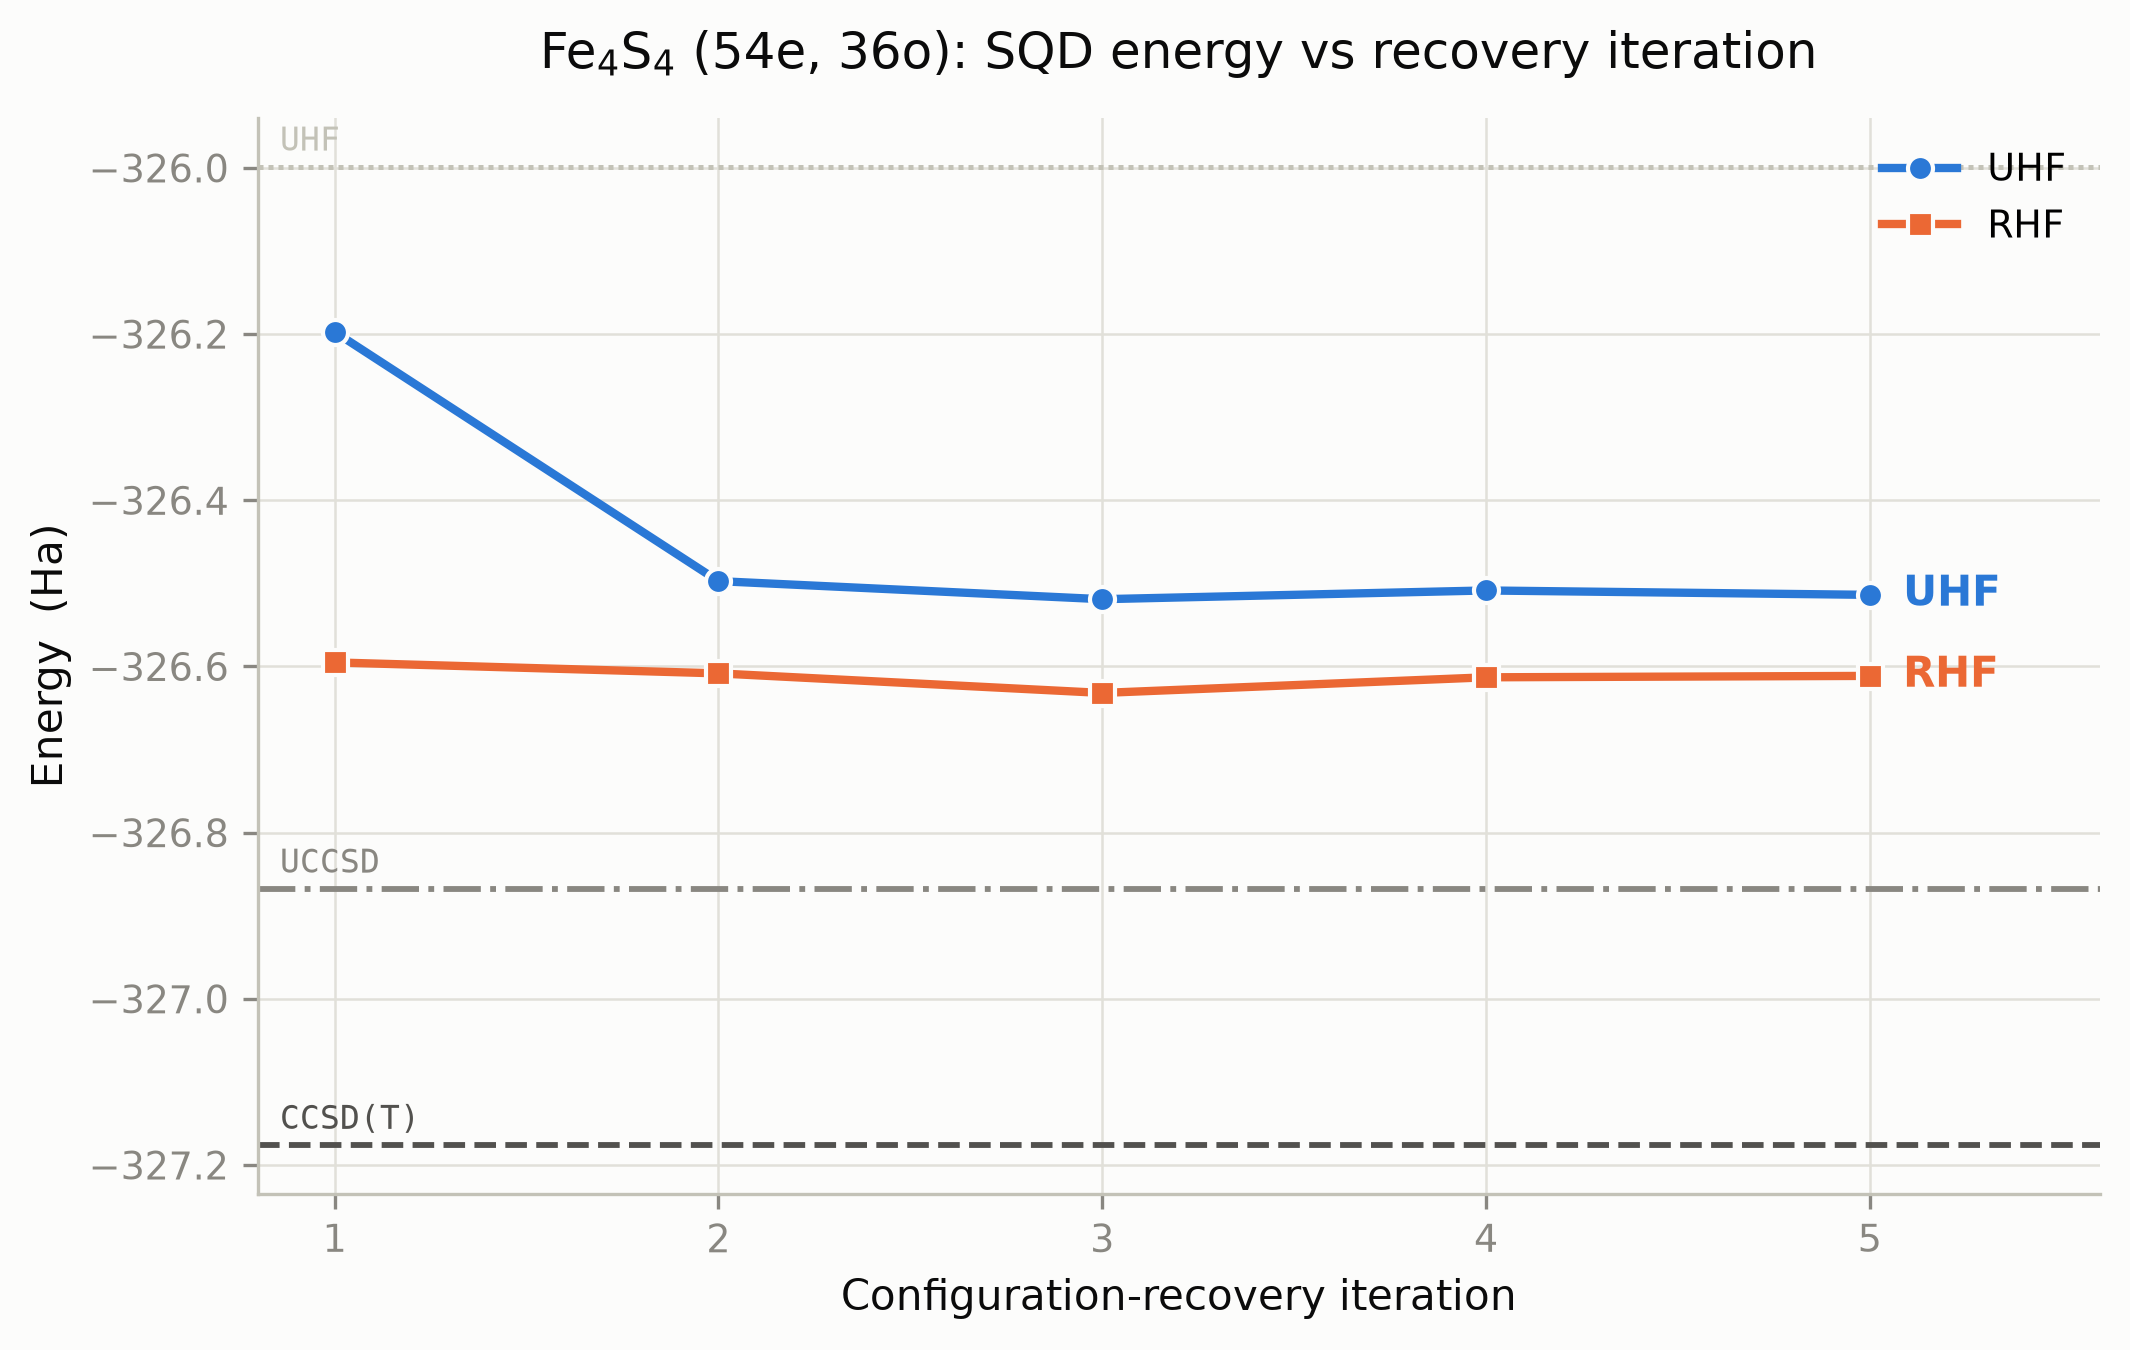
\includegraphics[width=0.9\textwidth]{fe4s4_rhf_vs_uhf.png}
\caption{\textbf{Fe$_4$S$_4$ (72q): RHF vs UHF SQD recovery} on GB200 GPU. Blue = UHF-SQD,
orange = RHF-SQD; both converge within $\sim$3 iterations, well below the UHF reference and
toward UCCSD/CCSD(T). \emph{[Figure: \texttt{fe4s4\_rhf\_vs\_uhf.png}]}}
\end{figure}

\subsection{Fe$_2$S$_2$ (40q): RHF vs UHF recovery, DMRG-anchored}
The same pipeline was run cleanly end-to-end on the smaller Fe$_2$S$_2$ active space (40 qubits,
30e/20o) on ROQUO GB200 GPU, with independent 5\,M-shot \texttt{ibm\_kobe} samples for each
reference and \texttt{sqd\_dim}$=3\times10^6$. We additionally computed a near-exact \textbf{DMRG}
reference (block2, bond dim $M$ up to 400+, $E_{\text{DMRG}}\approx-116.595$\,Ha).

\paragraph{Key finding --- coupled cluster is unreliable here.} Fe--S clusters are strongly
multireference, and it shows: CCSD(T) ($-116.375$) sits \textbf{$\sim$220\,mHa above the DMRG
ground state}, recovering only $\sim$52\,\% of the UHF$\to$DMRG correlation. So ``beating UCCSD''
is a weak statement --- CC itself is far from exact on this system. \textbf{DMRG is the only
trustworthy reference}, and all methods (SQD and CC alike) are benchmarked against it.

Against DMRG, both SQD results are variationally sound (safely above it) and \textbf{RHF-SQD
recovers as much correlation as CCSD(T)}: RHF-SQD captures $\sim$49\,\% of the UHF$\to$DMRG gap
($+234$\,mHa above DMRG) vs.\ CCSD(T)'s 52\,\% ($+220$\,mHa); UHF-SQD captures $\sim$30\,\%
($+324$\,mHa). RHF $>$ UHF is consistent with Fe$_4$S$_4$, but the honest picture is that a large
static-correlation gap remains beyond all of these methods at this subspace size.

\begin{table}[h]\centering
\begin{tabular}{@{}lrr@{}}
\toprule
Method & $E$ (Ha) & \% of UHF$\to$DMRG correlation \\
\midrule
UHF (reference) & $-116.135$ & 0\,\% \\
UHF-SQD (best)  & $-116.271$ & 30\,\% \\
UCCSD           & $-116.337$ & 44\,\% \\
RHF-SQD (best)  & $-116.361$ & 49\,\% \\
CCSD(T)         & $-116.375$ & 52\,\% \\
\textbf{DMRG (near-exact)} & $\mathbf{-116.595}$ & \textbf{100\,\%} \\
\bottomrule
\end{tabular}
\caption{Fe$_2$S$_2$ (40q): SQD (best over 5 recovery iterations, sqd\_dim $=3\times10^6$, GB200
GPU) vs classical references, anchored to DMRG. RHF-SQD $\approx$ CCSD(T) quality; CC is far from
exact (multireference). UHF-SQD trajectory: $-116.266,-116.270,-116.258,-116.271,-116.267$;
RHF-SQD: $-116.345,-116.361,-116.348,-116.321,-116.351$.}
\end{table}

\begin{figure}[h]\centering
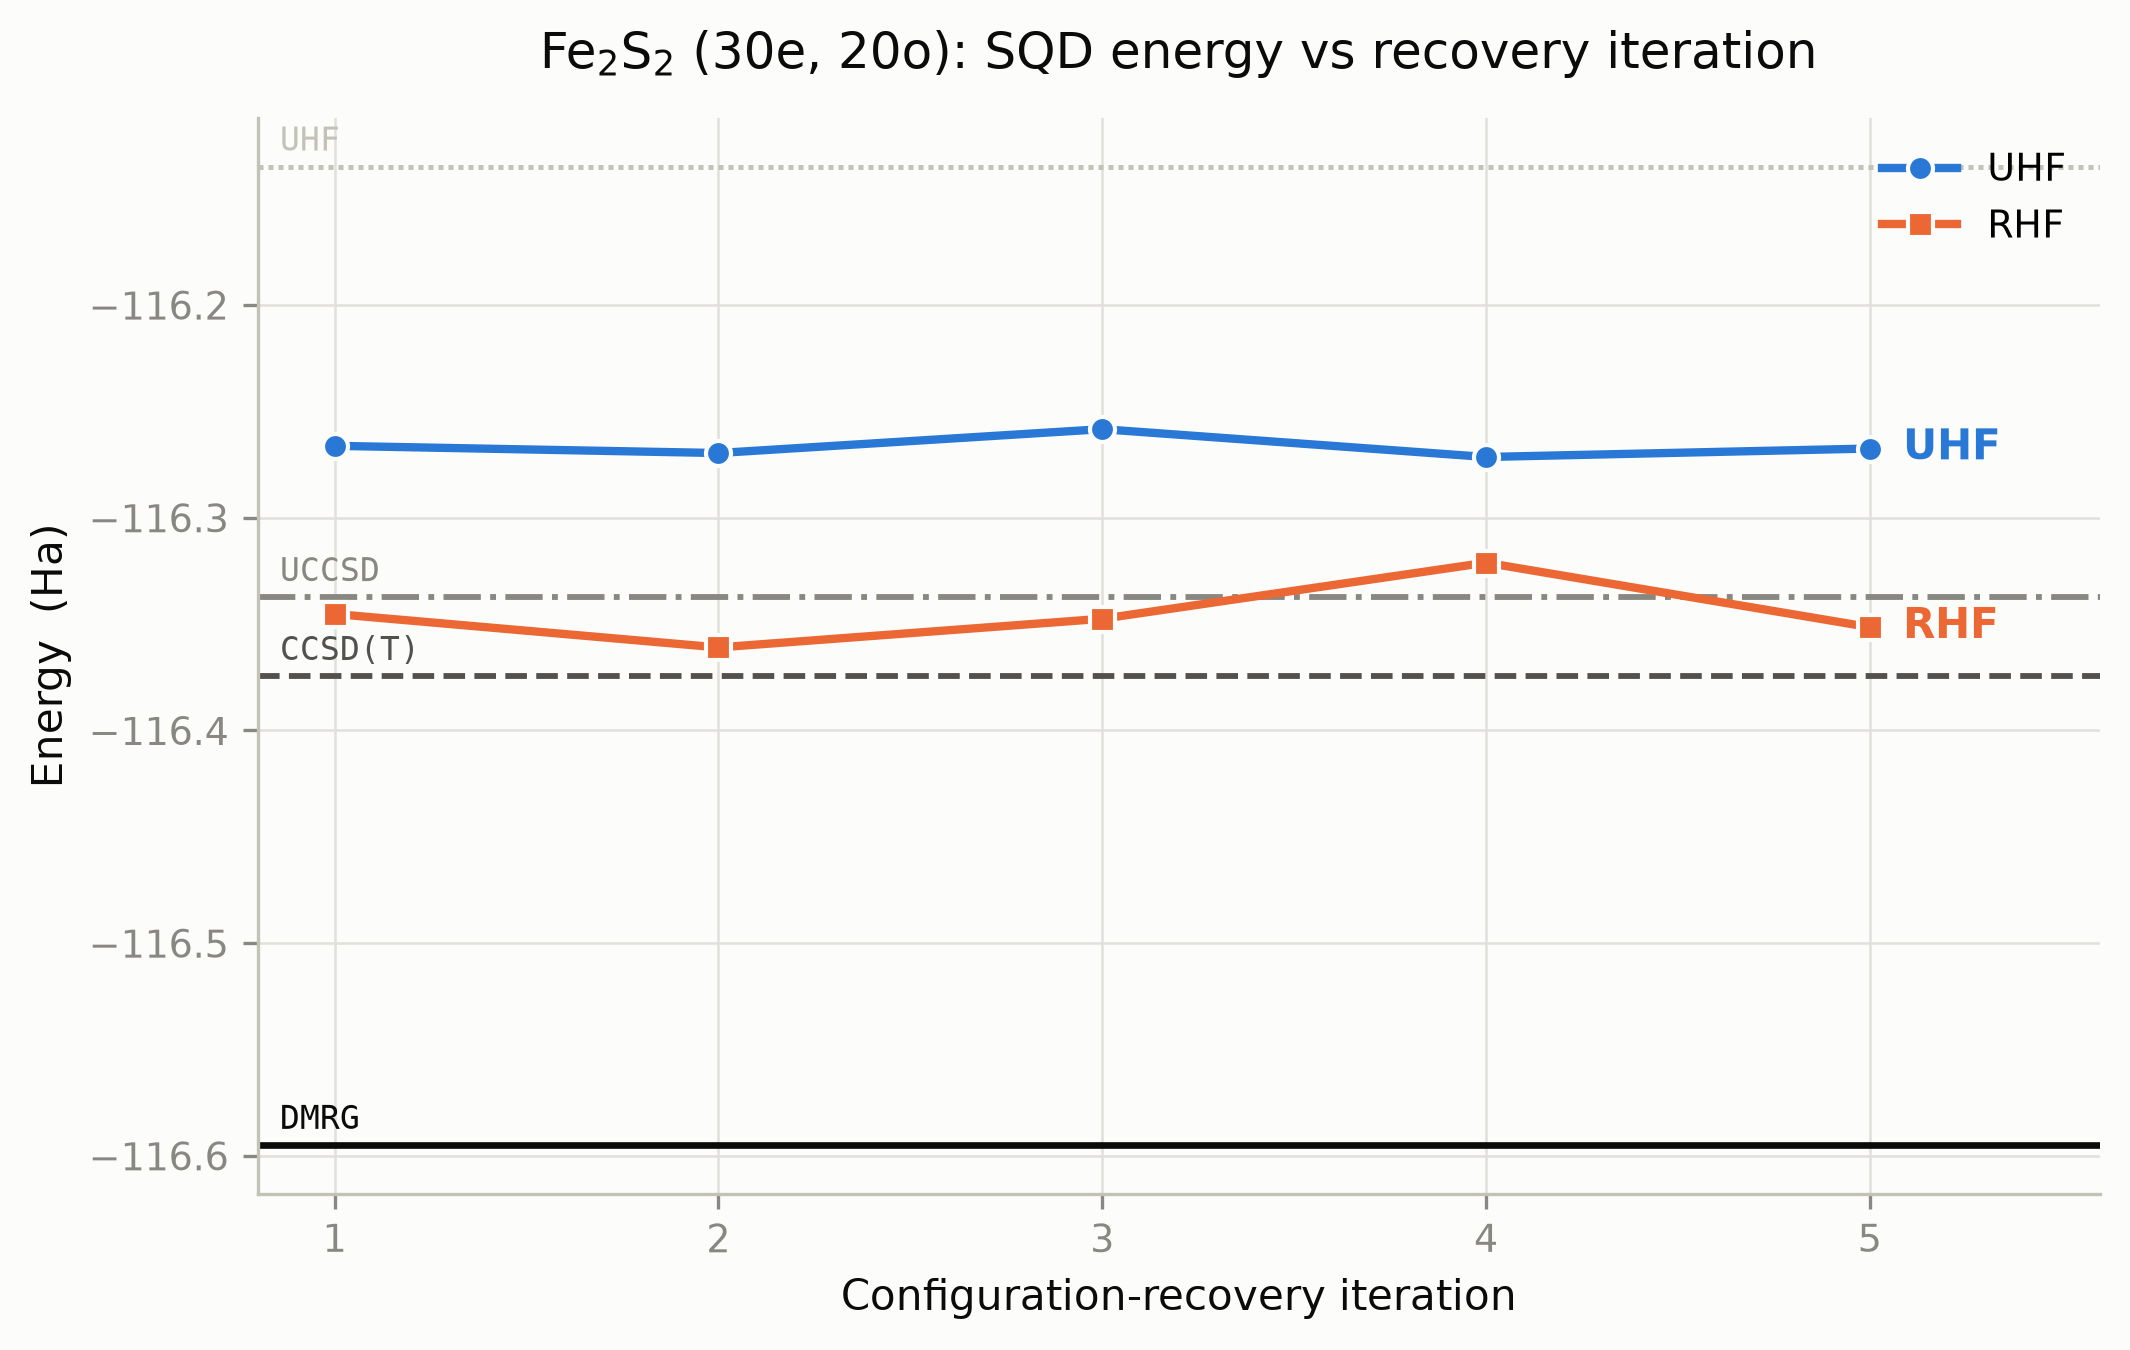
\includegraphics[width=0.9\textwidth]{fe2s2_energy_vs_iter.png}
\caption{\textbf{Fe$_2$S$_2$ (40q): RHF vs UHF SQD recovery} on GB200 GPU. Blue = UHF-SQD,
orange = RHF-SQD; horizontal lines are UHF (top), UCCSD, CCSD(T), and the near-exact DMRG anchor
(bottom, solid). The large DMRG--CCSD(T) gap exposes the coupled-cluster breakdown; RHF-SQD reaches
CCSD(T)-level correlation, UHF-SQD less, and substantial static correlation remains below all
curves. \emph{[Figure: \texttt{fe2s2\_energy\_vs\_iter.png}]}}
\end{figure}

% =====================================================================================
\section{Runtime summary and full hyperparameters}
% =====================================================================================
\subsection{Wall-clock (ROQUO, per job)}
All GPU jobs used the qtr node plan (1$\times$GB200, 36 cores). Sampling is dominated by the
IBM device queue + 5\,M-shot execution; recovery by the recover/subsample step and the GPU solve.
\begin{longtable}{@{}llrl@{}}
\toprule
Stage & System / method & Wall-clock & Notes \\
\midrule\endhead
Sampling (kobe, 5\,M shots) & Fe$_4$S$_4$ UHF & 41\,min & 1{,}312{,}655 kept shots \\
Sampling (kobe, 5\,M shots) & Fe$_4$S$_4$ RHF & 42\,min & $E_{\text{sample}}=-326.547$ \\
Sampling (kobe, 5\,M shots) & Fe$_2$S$_2$ UHF & 44\,min & $E_{\text{sample}}=-116.277$ \\
Recovery (5 iter, GB200)    & Fe$_4$S$_4$ UHF & 36\,min & $\sim$65--400\,s/solve, sqd\_dim $3\times10^8$ \\
Recovery (5 iter, GB200)    & Fe$_4$S$_4$ RHF & 27\,min & 1608\,s total flow \\
Recovery (5 iter, GB200)    & Fe$_2$S$_2$ UHF & 31\,min & sqd\_dim $3\times10^6$ (40q) \\
Recovery (5 iter, GB200)    & Fe$_2$S$_2$ RHF & 33\,min & 2007\,s total flow \\
Sampling (kobe, 5\,M shots) & Fe$_2$S$_2$ RHF & 51\,min & \\
Single GPU solve (17{,}320 dets/spin) & Fe$_4$S$_4$ & 13--65\,s & Davidson $\sim$13--24\,s + FCIDUMP parse/GPU init \\
References (UHF/UCCSD/CCSD(T)) & Fe$_4$S$_4$ (36o) & $\sim$30\,min & CCSD(T) triples dominate \\
References (UHF/UCCSD/CCSD(T)) & Fe$_2$S$_2$ (20o) & $\sim$5\,min & \\
GPU build (nvc++, both binaries) & --- & $\sim$8\,min & one-time, on a compute node \\
\bottomrule
\end{longtable}

\subsection{Complete hyperparameter set}
Identical for UHF and RHF except \texttt{--method} (and hence the reference, LUCJ ansatz, and diag
binary). Fe$_2$S$_2$ uses the same values except \texttt{sqd\_dim} (see note).
\begin{longtable}{@{}lll@{}}
\toprule
Parameter & Value & Meaning \\
\midrule\endhead
\multicolumn{3}{@{}l}{\emph{Active space / problem}}\\
\ \ Fe$_4$S$_4$ & NORB=36, NELEC=54, MS2=0 & 72 qubits, singlet \\
\ \ Fe$_2$S$_2$ & NORB=20, NELEC=30, MS2=0 & 40 qubits, singlet \\
\ \ \texttt{method} & \texttt{uhf} $|$ \texttt{rhf} & reference determinant / diagonalizer \\
\midrule
\multicolumn{3}{@{}l}{\emph{Quantum sampling (IBM \texttt{ibm\_kobe})}}\\
\ \ \texttt{shots} & 5{,}000{,}000 & total measurement shots \\
\ \ \texttt{n\_shot\_batches} & 5 & $5\times10^6$ split into 5$\times$1\,M (\texttt{concatenate\_shots}) \\
\ \ \texttt{quantum\_source} & \texttt{real-device} $\to$ \texttt{saved} & sample once, reuse the pool \\
\ \ dynamical decoupling & on, sequence \texttt{XY4} & error mitigation \\
\ \ measurement twirling & on & error mitigation \\
\ \ gate twirling & off & (fails on fractional LUCJ \texttt{rzz}) \\
\ \ reset mitigation & on & \\
\midrule
\multicolumn{3}{@{}l}{\emph{LUCJ circuit (ansatz)}}\\
\ \ \texttt{n\_lucj\_layers} & 1 & reduces noise at high qubit count \\
\ \ ansatz seed & (U)CCSD amplitudes & \texttt{SEED\_CCSD\_MAX\_CYCLE=200} + DIIS \\
\ \ transpiler opt.\ level & 3 & SABRE layout (1024 trials, 8 iters, 10 swap trials) \\
\midrule
\multicolumn{3}{@{}l}{\emph{Configuration recovery / SQD}}\\
\ \ \texttt{sqd\_dim} & $3\times10^8$ (Fe$_4$S$_4$); $3\times10^6$ (Fe$_2$S$_2$) & subspace dim ($\sqrt{}\!\approx$17320 / 1732 dets/spin) \\
\ \ \texttt{n\_recovery\_steps} & 5 & self-consistent configuration-recovery passes \\
\ \ \texttt{n\_batches} & 1 & K-batch count (1: concurrent GPU solves OOM) \\
\ \ \texttt{carryover\_type} & 1 & determinant carryover enabled \\
\ \ \texttt{carryover\_ratio} & 0.5 & \\
\ \ Hamming post-selection & $(N_\alpha,N_\beta)$ sector & fixes particle number / $S_z$ \\
\midrule
\multicolumn{3}{@{}l}{\emph{Differential evolution (single-pass eval)}}\\
\ \ \texttt{num\_walkers} & 1 & single evaluation pass \\
\ \ \texttt{iterations} & 1 & no DE optimization loop \\
\ \ \texttt{randomization\_factor} & 0.2 & ansatz perturbation from CCSD \\
\ \ \texttt{fxc} & 0.5 & DE scaling factor (unused at 1 walker) \\
\midrule
\multicolumn{3}{@{}l}{\emph{ROQUO GPU execution}}\\
\ \ \texttt{hpc\_target} & \texttt{slurm} & per-solve \texttt{sbatch} + \texttt{sacct} poll \\
\ \ \texttt{solver\_mode} & \texttt{gpu} & selects \texttt{diag-gpu}/\texttt{diag-gpu\_uhf} \\
\ \ \texttt{--slurm-gres} & \texttt{gpu:1} & one GB200 per solve (multi-rank OOMs) \\
\ \ launcher / MPI opts & \texttt{srun} / \texttt{--gpu-bind=closest} & PMIx, 1 rank/GPU \\
\ \ modules & \texttt{cuda/13.2}, \texttt{hpcx/2.50} & \\
\ \ \texttt{ompthreads} & 36 & qtr-plan host cores \\
\ \ \texttt{solver\_timeout\_seconds} & 43{,}200 & 12\,h \\
\ \ \texttt{walltime} & 3--4\,h & \\
\midrule
\multicolumn{3}{@{}l}{\emph{Classical references}}\\
\ \ SCF / CCSD \texttt{max\_cycle} & 300 & + DIIS(12) + level-shift(0.2) for hard Fe--S \\
\ \ HCI & skipped ($>$24 orbitals) & selected-CI intractable at 72q \\
\ \ DMRG & deferred (block2) & near-exact anchor, separate job \\
\midrule
\multicolumn{3}{@{}l}{\emph{GPU build}}\\
\ \ compiler & \texttt{nvc++} 26.5 & \texttt{-std=c++17 -mp -cuda -fast -gpu=mem:unified,cc100 -DSBD\_THRUST} \\
\ \ arch & \texttt{cc100} (sm\_100) & GB200 Blackwell \\
\midrule
\multicolumn{3}{@{}l}{\emph{Prefect robustness (ROQUO)}}\\
\ \ \texttt{PREFECT\_API\_REQUEST\_TIMEOUT} & 600\,s & long child-solve polls exceed 60\,s default \\
\ \ \texttt{PREFECT\_HOME} & Lustre (\texttt{/home}) & pool + DB persistence \\
\ \ task runner / telemetry & Concurrent / disabled & avoid SQLite contention \\
\bottomrule
\end{longtable}

% =====================================================================================
\section{Commit history}
% =====================================================================================
All work is on branch \texttt{kk/feature/uhf} over the six-day window (2026-07-01 to 2026-07-08).
Core library edits are committed; the experiment scratch (\texttt{algorithms/sbd/sweep/}) is
intentionally untracked (synced to HPC via \texttt{scp}). All 48 commits are listed below,
grouped by theme (oldest first).

\begin{longtable}{@{}lp{0.78\textwidth}@{}}
\toprule
Commit & Change \\
\midrule\endhead
\multicolumn{2}{@{}l}{\emph{Foundations: solver + recovery + saved-pool source}}\\
\texttt{12a4232} & Stop dumping \texttt{matrixformwf.txt} from the SBD solver \\
\texttt{1a63b31} & Add \texttt{carryover\_type} flag to actually enable determinant carryover \\
\texttt{aac6a3f} & Guard shot-batch reset mitigation against an empty kept set \\
\texttt{0361bae} & Allow \texttt{num\_walkers} below 4 for single-pass evaluation runs \\
\texttt{b91dde5} & Expose solver wait timeout as a \texttt{create\_blocks} knob \\
\texttt{b9023b1} & Persist merged sample pool and add a saved-samples source (``sample once, reuse'') \\
\midrule
\multicolumn{2}{@{}l}{\emph{Recovery harness + Slurm/ROQUO enablement}}\\
\texttt{d4747b3} & Fe2S2 RHF-vs-UHF recovery harness + per-step \texttt{recovery\_trace} \\
\texttt{9e9d73d} & Add \textbf{Slurm} \texttt{hpc-target} to \texttt{create\_blocks} + ROQUO RHF launcher \\
\texttt{886d8ff} & Point ROQUO RHF launcher at the transferred FCIDUMP path \\
\texttt{43699d2} & Prefect ephemeral DB on node-local tmp for ROQUO run \\
\texttt{34c261f} & Add \texttt{local} hpc-target; run solver in-allocation (no per-solve sbatch) \\
\texttt{995474c} & Fix SQLite lock: ConcurrentTaskRunner + long DB timeout \\
\texttt{34205f7} & Parametrize sweep harness by molecule (fe2s2 $|$ fe4s4) \\
\midrule
\multicolumn{2}{@{}l}{\emph{Fe4S4 72q sampling (Fugaku, kobe)}}\\
\texttt{6e7e3bf} & Add Fe4S4 72q Fugaku sampling launcher (5M shots, kobe) \\
\texttt{c314521} & Lint fixes in Fe4S4 sample launcher \\
\texttt{86e8dba} & Fe4S4 sampling: UHF + large-node grid, disable telemetry, PJM orchestrator \\
\texttt{4389188} & Fe4S4 sampling: default 60$\times$60 = 3600-node grid \\
\texttt{230d364} & Fe4S4 sampling: PJM group \texttt{ra010014} + gfscache directives \\
\texttt{1117f24} & Fe4S4 sampling orchestrator on mem2 (x86\_64); CCSD convergence controls \\
\texttt{aef75f3} & Fe4S4 recovery from saved kobe pool (3e8, rec5) + data-area work dirs \\
\midrule
\multicolumn{2}{@{}l}{\emph{ROQUO GB200 GPU: build + launch + memory/OOM fixes}}\\
\texttt{160d27d} & Add ROQUO GB200 GPU recovery runner (\texttt{diag-gpu}) \\
\texttt{e44d6e1} & Fix GPU launch: \texttt{mpirun} (diag-gpu is MPI) \\
\texttt{ee60ab6} & GPU: run \texttt{diag-gpu} on 1 GPU (multi-rank OOMs) \\
\texttt{523e04b} & Add ROQUO RHF sampling runner (kobe from compute node) \\
\texttt{44b721a} & Lint fixes in ROQUO RHF sampler \\
\texttt{f7b9011} & GPU: \texttt{n\_batches=1} (fix concurrent-GPU OOM) + scratch work dir \\
\texttt{596f8c6} & Lint: shorten comment lines in GPU runner \\
\texttt{1599d36} & refs: guard empty \texttt{DMRG\_M} \\
\texttt{65bb8fa} & GPU: keep solver work\_dir on Lustre (\$SLURM\_SCRATCH breaks diag-gpu) \\
\texttt{4830d6d} & Lint: drop unused Path import, shorten comment \\
\midrule
\multicolumn{2}{@{}l}{\emph{Slurm-target GPU (per-solve sbatch) + refs/plot fixes}}\\
\texttt{a6c13ef} & \textbf{Slurm target GPU support} (\texttt{--gres}, \texttt{srun}/PMIx) \\
\texttt{4c474ac} & Pass \texttt{srun/--gpu-bind} via env (argparse rejects \texttt{--flag} opts) \\
\texttt{16d1439} & refs: fix \texttt{mycc.e\_tot()} $\to$ \texttt{e\_tot} \\
\texttt{3f2d662} & slurm template: \texttt{unset SLURM\_CPUS\_PER\_TASK/TRES} before nested srun \\
\texttt{c013ac3} & GPU runner: scan all telemetry artifacts for \texttt{recovery\_trace} \\
\texttt{1dfdbdd} & GPU runner: \texttt{PREFECT\_API\_REQUEST\_TIMEOUT=600} (multi-step httpx fix) \\
\texttt{ca869dd} & refs: skip HCI above \texttt{HCI\_MAX\_NORB} (hangs at 72q) \\
\texttt{53fea0b} & RHF sampler: \texttt{PREFECT\_HOME} on Lustre so the pool persists \\
\midrule
\multicolumn{2}{@{}l}{\emph{Figures, cleanup, presentation}}\\
\texttt{00030b5} & plot: molecule-aware output filenames \\
\texttt{05c192c} & plot: error panel falls back to CCSD(T)/UCCSD when no DMRG \\
\texttt{aa20e57} & cross-system \%-recovered figure \\
\texttt{e1e82f3} & Untrack \texttt{algorithms/sbd/sweep/}; gitignore experiment scratch \\
\texttt{2a7eba9} & docs: Overleaf presentation summary + Fe4S4/Fe2S2 figures \\
\texttt{448293c} & docs: RHF-vs-UHF Fe4S4 results + runtime \& full hyperparameter tables \\
\texttt{79434d4} & docs: refresh two-panel (Fe4S4 shows both UHF+RHF curves) \\
\texttt{0b2d7fc} & docs: Fe2S2 panel now a UHF recovery curve (was single point) \\
\texttt{a15de7d} & docs: complete Fe2S2 RHF-vs-UHF results + all-four-trajectory figures \\
\bottomrule
\end{longtable}

\section{Summary}
The SQD closed loop now runs natively on ROQUO GB200 GPUs through Prefect's Slurm target, with a
GPU-accelerated selected-CI solver. The complete RHF-vs-UHF recovery comparison was obtained on
\emph{both} iron--sulfur active spaces: Fe$_2$S$_2$ (40 qubits) and Fe$_4$S$_4$ (72 qubits). In
every case the configuration-recovery loop converges within $\sim$3 iterations, pulling the energy
several hundred mHa below the UHF reference; the restricted (RHF) reference recovers deeper than the
unrestricted (UHF) one in both systems. Best recovered energies (Ha): Fe$_2$S$_2$ UHF $-116.271$ /
RHF $-116.361$; Fe$_4$S$_4$ UHF $-326.519$ / RHF $-326.632$.

Anchoring to a near-exact \textbf{DMRG} reference (Fe$_2$S$_2$: $-116.595$\,Ha) reframes the
comparison honestly: these Fe--S active spaces are strongly multireference, so \textbf{CCSD(T)
itself is $\sim$220\,mHa from exact} and is not a reliable yardstick. Measured against DMRG,
RHF-SQD reaches CCSD(T)-level correlation ($\sim$49\,\% of the UHF$\to$DMRG gap vs CCSD(T)'s
52\,\%) and UHF-SQD less ($\sim$30\,\%), with substantial static correlation remaining beyond all
methods at this subspace size. The Fe$_4$S$_4$ (72q) DMRG anchor is in progress. Every step --- GPU
build, sampling, pool persistence, multi-iteration recovery, references (incl.\ DMRG), and figures
--- is reproducible from the commands above; all figures are in \texttt{docs/2026-07-08/figures/}.

\end{document}
